\documentclass[10pt,journal,compsoc]{IEEEtran}

\usepackage[pdftex]{graphicx}    
\usepackage{cite}
\usepackage{listings}
\usepackage{subcaption} 
\usepackage{dirtree}
\usepackage{mathtools}
\hyphenation{op-tical net-works semi-conduc-tor}
\graphicspath{ {../images/} }


\begin{document}
	
\title{Robotics Software Engineer Nanodegree: Slam Project}
\author{Manuel Huertas L\'opez}

\markboth{Slam project, Udacity}{}
\IEEEtitleabstractindextext{%
	
\begin{abstract}
Simultaneous localization and mapping, SLAM, is the problem of building a map of an unknown environment while simultaneously localize a robot relative to this map. In this project a 2D and 3D occupancy grid map was created from both a simulated environment provided by the Udacity team and an environment that was created from scratch. A robot with two differential drives and equipped with a Lidar and a RGB-D camera was used in the simulated environment.The library RTAB-Map was selected to solve the slam problem because: it offers a good performance and memory management, a good portfolio of development tools, and a good quality of the documentation. 
\end{abstract}


\begin{IEEEkeywords}
slam, udacity, rtab-map.
\end{IEEEkeywords}}
	
	
\maketitle
\IEEEdisplaynontitleabstractindextext
\IEEEpeerreviewmaketitle
\section{Introduction}
\label{sec:introduction}
\IEEEPARstart
{T}{here} are some applications where a Robot is provided with a map of its environment and it is able to estimates its pose based on this map, the odometry data and some sensor data like a Lidar or RGB-D camera. Furthermore, in some case the map is unknown, either because the area is unexplored or because the surrounding change often and the map may not be updated. In that case the Robot must construct a map, the Robot's pose is known and the Robot is equipped with sensor data to measure its environment. There are several difficulties when building a map: high dimensionality of the space, size, noise, perceptual ambiguity , Robot moving in cycles. The  high dimensionality problem can be overcome by using an occupancy grid map where the space is represented by a fine-grained grid over the continuous space in the environment. The noise or incertains is manages by using probabilistic estimations. Finally, in the most general case neither the Robot's pose and map is available, this is where slam cames in. In slam, the Robot will use the odometry and the sensor data to build a map of its environment while simultaneously localize itself relative to this map. The slam problem is quite challenging, with noise in the Robot pose and measurement, the Robot's pose will be uncertain and the construction of the map will be uncertaion as well, they are interrelated. This project will use an implementation of slam called real time appearance based mapping or RTABmap. This implementation is based on Graph Slam. GraphSlam is a slam algorithm that solves the full slam problem, this means that the algoritm recovers the entire path and map, instead of just the most recent pose and map.
\section{Background / Formulation}
The SLAM problem is considered the most fundamental problem in robotics. It is considered as a prerequisite for truly autonomous robot navigation. In the following section two different algorithms are explained. For the project the Graph SLAM algorithm was selected since it has both a better performance and accuracy.
\subsection{Grid-based FastSLAM}
FastSLAM algorithm uses the particle filter approach along with the low dimensional extended Kalman filter to incrementally estimate the posterior distribution over Robot pose along with the positions of some landmarks. FastSLAM decomposes the SLAM problem into a Robot localization problem, and a collection of landmark estimation problems that are conditioned on the Robot pose estimate. In order to solve the SLAM problem FastSlam uses a modified particle filter for estimating the posterior over Robot path, for every particle in the filter there are K Kalman filters that estimate the K landmark locations conditioned on the path estimate. An implementation of this idea requires {O(MK)} time, where M is the number of particles and K the number of landmarks, by using a tree-based data structure the running time can be reduced to {O(MlogK)}. Finally, there are different versions of the algorithm. The one used during the course is called Grid-based FastSLAM which adapts FastSLAM to grid maps with the main advantage of no need for predefining landmark, that means it will work in arbitrary environments.

\begin{align}
p(x_{0:t},m|z_{1:t},u_{1:t})=p(x_{0:t}|z_{1:t},u_{1:t})p(m|x_{1:t},z_{1:t})
\end{align}

The Grid-base FastSLAM use three different techniques: sampling motion, map estimation and importance weight.

In the sample motion technique estimates the current pose given the K-th particles previous pose a the current controls.
\begin{align}
p(x_{t}|x_{t-1}^{[k]},u_{t})
\end{align}
The map estimation technique goal is to estimate the current map giving the current measurement, the current K-th particle pose and the previous K-th particle map. The occupancy grid mapping algorithm is used at this stage.
\begin{align}
p(m_{t}|z_{t},x_{t}^{[k]},m_{t-1}^{[k]})
\end{align}
Finally, the importance weight technique which compute the importance weight of each individual particle.
\begin{align}
p(z_{t}|x_{t}^{[k]},m^{[k]})
\end{align}

\subsection{GraphSLAM}
GraphSLAM uses constraints to represent relationships between Robot poses and the environment, and then tries to resolve all of these constraints to create the most likely map given the data. GraphSLAM solves the full slam problem. Furthermore, GraphSLAM has several advantages over FastSLAM including the reduced need for onboard processing capability and an important improvement in accuracy since FastSLAM uses particles and it can happen that there is no particle in the actual pose of the Robot. 

In GraphSLAM the problem is decoupled in two tasks: to create a graph of all Robot poses and features in the scene and to find the most likely Robot's path and map of the environment. These two tasks are called Front-End and Back-End.

The Front-End of GraphSLAM constructs the graph using the odometry and sensory measurements collected by the Robot. This is done continuously as the Robot moves around the environment. This step can vary greatly from application to application depending on the desire accuracy, the Robot sensors etc. In this step the features in the environment that have been previously seen are treated. 

The input of the Back-End is the complete graph with all the constraints that have already been built in the previous step. The output is the most probable configuration of the Robot poses and map features. It takes all the constraints and calculates the configuration that produces the smallest error. It is more consistent between different applications. This two-step can be applied iteratively.
\section{Scene and robot configuration}
\subsection{World}
A world in gazebo was created from scratch using a floor plan. Walls, doors and windows were added. Finally, few objects were put in the scene using the gazebo model editor. The result can be seen in the following figure.
\begin{figure}[h]
\centering
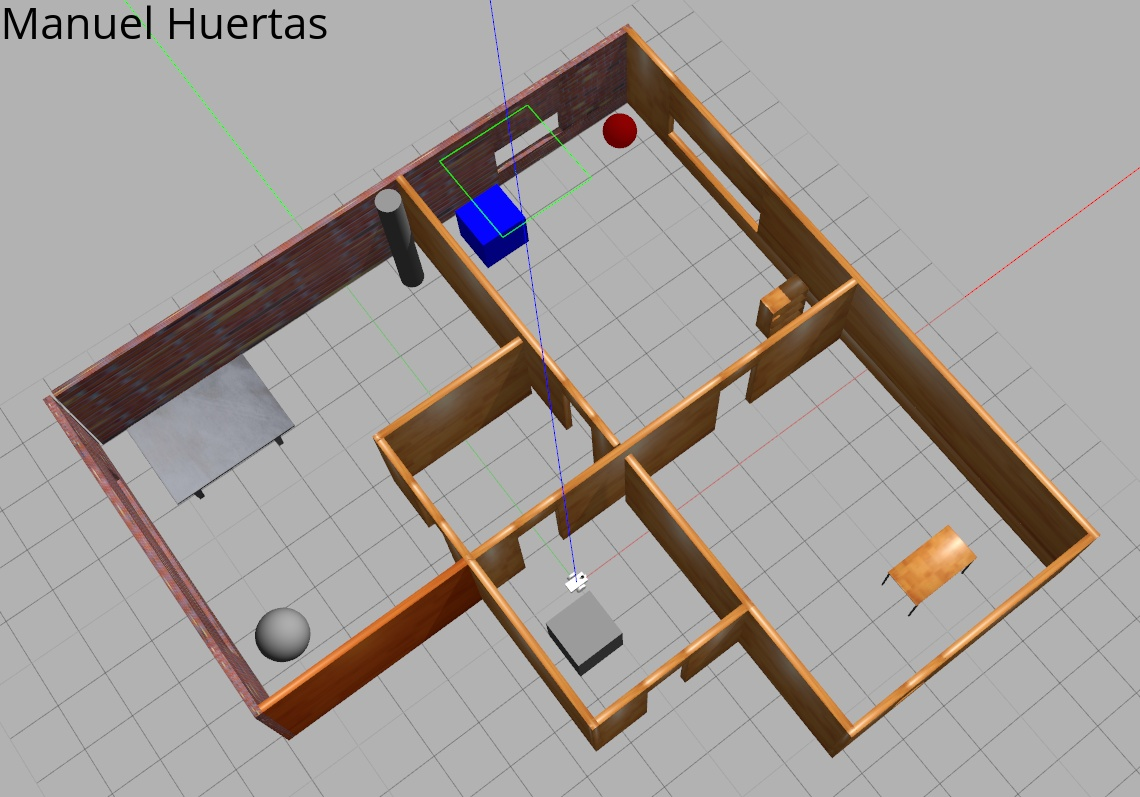
\includegraphics[scale=0.20]{robot-own-world}
\caption{Robot own world.}
\label{fig:world}
\end{figure}
\subsection{Robot}
The model provided by Udacity is a 2W robot with two caster, one on the front and another on the back, to stabilise. A Lidar and a camera were added at the front, for the navigation stack. The inertial and friction parameters where adjusted in order to give a smooth movement to the robot. The robot was modified to include a RGB-D camera, kinect, in order to produce a 2D and 3D maps of the scene.
\begin{figure}[h]
\centering
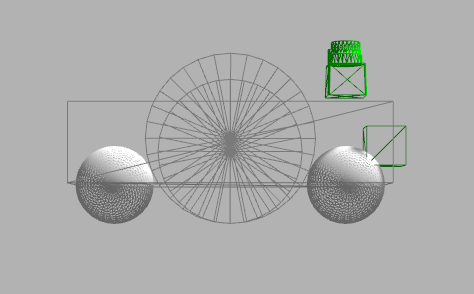
\includegraphics[scale=0.33]{udacity-design-2}
\caption{Udacity design view.}
\label{fig:mesh1}
\end{figure}
\begin{itemize}
\item Chassis: a box of size 40cm x 20cm x 1cm.
\item Wheels: two wheels 1cm x 0.5cm located in the front of the platform.
\item Casters: two caster one the back and another on the front.
\item Lidar: a hokuyo lidar in the front.
\item Camera: a RGB-D camera in the head of the platform
\end{itemize}
\subsection{Packing Structure}
A module named slam\_project was created with the follwing structure:
\dirtree{%
.1 slam\_project.
.2 CMakeLists.txt.
.2 config.
.2 launch.
.2 meshes.
.2 package.xml.
.2 scripts.
.2 urdf.
.2 worlds.
}
Three different launchs files were created:
roslaunch slam\_project world.launch
roslaunch slam\_project teleop.launch
roslaunch slam\_project mapping.launch
roslaunch slam\_project rviz.launch
\section{Results}


\begin{figure}[h]
\centering
\begin{subfigure}[b]{0.2\textwidth}
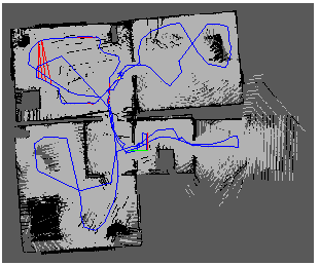
\includegraphics[scale=0.3]{own-occupancy-grid-map}
\caption{Occupancy Grid Map}
\end{subfigure}
\begin{subfigure}[b]{0.2\textwidth}
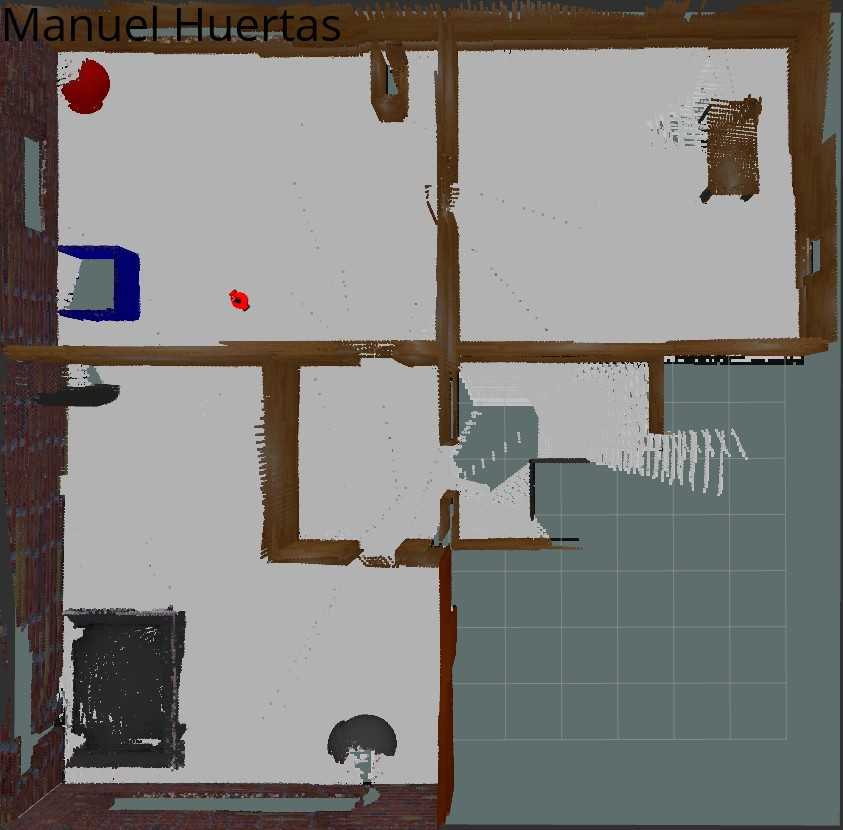
\includegraphics[scale=0.3]{own-3d-map}
\caption{3D octomap}
\end{subfigure}
\caption{Own world}
\end{figure}








\section{Discussion}
\section{Conclusion / Future work}

\begin{thebibliography}{9}
\bibliographystyle{ieeetr}

\bibitem{udacity} 
https://eu.udacity.com
\textit{Robotics Software Engineer Nanodegree program}. 

\bibitem{deeplearning} 
Adit Deshpande
\textit{The 9 Deep Learning Papers You Need To Know About}. 

\bibitem{analysisdnn} 
Alfredo Canziani, Eugenio Culurciello,Adam Paszke  
\textit{An analysis of deep neural network models for practical applications}. 
\end{thebibliography}
\end{document}
	
	

